\chapter{Vector-Like Quarks (VLQs) }
\epigraph{\itshape The longer I live, the more uninformed I feel. Only the young have an explanation for everything.}{Isabel Allende, \textit{The City of the Beasts} }

\epigraph{\itshape There is a theory which states that if ever anyone discovers exactly what the Universe is for and why it is here, it will instantly disappear and be replaced by something even more bizarre and inexplicable. There is another theory which states that this has already happened.}{Douglas Adams, \textit{The Restaurant at the End of the Universe}}

The gauge hierarchy problem (sec.~\ref{gaugeHprob}) is caused by a quadratic divergence in the Higgs self-energy. One way to address this problem is to extend the Higgs sector. This can be achieved in several approaches, the two highlighted here are: compositeness of the Higgs boson and extending the Higgs sector with an extra dimension.

In composite Higgs models \cite{Kaplan}, the Higgs boson is a bound state and fermions have high mass partners. In early versions of this model, fermions were hypothesized to exist in a partially composite state where fermions become a linear combination of a light mass and heavy mass state predicting the existence of high mass resonances. Later versions focused on developing a mechanism around the top quark wherein the top has a heavier partner. In both cases, a fourth generation of non-chiral quarks arises \cite{compositeHiggs}.

In little Higgs models, the Higgs boson is a pseudo-Goldstone boson and a symmetry breaking at the TeV scale is added. This symmetry breaking gives rise to the light Higgs boson and eliminates the problematic radiative corrections. Like the composite Higgs models, these theories also predict the existence of a top partner \cite{littleHiggs}.

In all of these theories, a new fourth generation of quarks must have left- and right-handed weak eigenstates with the same weak quantum numbers. These new quarks will couple to heavy quarks, have colour charge, and have fractional charge. It is these properties that have motivated the name Vector-Like Quarks (VLQs).

VLQs are appealing in many ways. In addition to solving the gauge hierarchy problem, VLQs also provide new sources of CP violation. This will help to further explain the matter anti-matter asymmetry observed in our universe. VLQs are ascetically nice providing a fourth generation in the standard model. A chiral fourth genration has already been ruled out experimentally, so VLQs are the simplest way of adding a fourth generation to the standard model \cite{VLQHandbook}. 

Extensions of the Higgs sectors are not the only theories that predict the existence of vector-like fermions. Hypothetically speaking, vector-like fermions could be added to the standard model without addressing the gauge hierarchy problem. However, the VLQs in these theories arise from extending the Higgs sector yielding predictions that have unique experimental consequences.

\section{Symmetry Breaking in the "Littlest Higgs"}

VLQs do not obtain their mass from a Yukawa coupling to the Higgs field. Instead, the mass is the result of a broken symmetry. In all of the composite Higgs and little Higgs models, there is some higher symmetry that is broken. This section will focus on the method of symmetry breaking presented in the "littlest Higgs" model \cite{littleHiggs}.

The gauge hierarchy problem is specifically concerned about the large difference in $m_{h}^{2} / \Lambda^{2}$ where $\Lambda$ is the cutoff scale, which is $10^{16}$ GeV in the standard model. But, what if there is another broken symmetry which has a cutoff around $\Lambda=10^{4}$ GeV? This is a much more manageable scale. In the littlest Higgs model, a higher $SU(5)$ symmetry with this lower cutoff scale is proposed. This symmetry breaks $SU(5)\rightarrow SO(5)$ creating 14 Goldstone bosons. These bosons are "eaten" creating the electroweak and Higgs bosons that we observe \cite{littleHiggs}.

This is achieved by considering the $SU(5)$ subgroup $G_{1}\times G_{2}=[SU(2)\times U(1)]^{2}$, which is broken to give rise to the electroweak gauge symmetry $SU(2)\times U(1)$. This model has the Lagrangian
\begin{equation}
    \mathcal{L} = \mathcal{L}_{K} + \mathcal{L}_{t} + \mathcal{L}_{\psi}
\end{equation}
where $\mathcal{L}_{K}$ are the kinetic terms, $\mathcal{L}_{t}$ is the origin of the top Yukawa coupling, and $\mathcal{L}_{\psi}$ creates the other Yukawa couplings. The term $\mathcal{L}_{t}$ shows the origin of VLQs in this model
\begin{equation}
    \mathcal{L}_{t} = \lambda_{1}(q_{3}h+f\Tilde{t})u_{3}^{'c} + \lambda_{2}f\Tilde{t}\Tilde{t}^{c} + ...
\end{equation}
This results in a heavy fermion $\Tilde{t}$ that is multiplied by a linear combination of $u_{3}^{'c}$ and $\Tilde{t}^{c}$. It also yields the top Yukawa coupling
\begin{align}
    \lambda_{t}q_{3}hu_{3}^{c} & \textrm{ where } \lambda_{t}=\frac{\lambda_{1}\lambda_{2}}{\sqrt{\lambda^{2}_{1}+\lambda^{2}_{2}}}
\end{align}
The heavy fermion gives a negative contribution to the Higgs mass
\begin{equation}
    -\frac{3\lambda^{2}_{t}}{8\pi^{2}}m^{'2}\textrm{log}\frac{\lambda^{2}}{m^{'2}}
\end{equation}
When this negative mass term dominates over the positive mass terms it triggers electroweak symmetry breaking \cite{littleHiggs}. 

In this theory, the fermions become $(5,3)$ and $(5,\bar{3})$ multiplets under $SU(5)\times SU(3)_{\textrm{color}}$ The top and bottom quark become a mixture of a $(5,3)$ multiplet and a new quark doublet field $q$, while the anti-top is a mixture of a $(5,\bar{3})$ multiplet and the $SU(5)$ singlet field $t^{c}$. The $q$ and $t^{c}$ fields induce the symmetry breaking and give rise to a Higgs boson with a physical mass consistent with the observed mass of $125$ GeV. All of this, while avoiding quadratic divergences \cite{littleHiggs}. An example of the new VLQ loop contributions to the Higgs mass is shown in Fig.~\ref{fig:tprimeLoop}

\begin{figure}[htb]
    \centering
    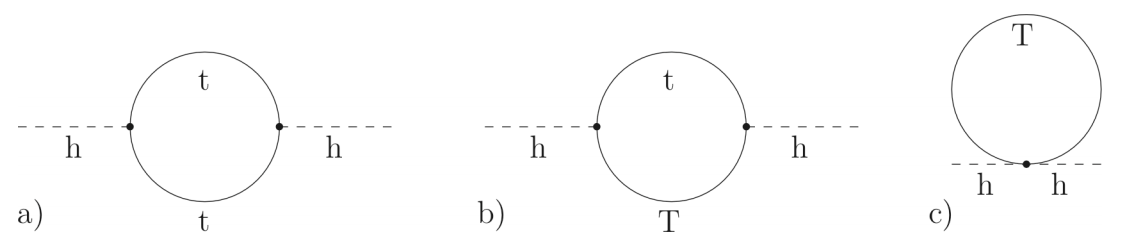
\includegraphics[width=14cm]{tprimeLoop.png}
    \caption{The top partner loop contributions to the Higgs mass in the littlest Higgs model. From \cite{TopPartner}}
    \label{fig:tprimeLoop}
\end{figure}

In this theory, the VLQs arise as a doublet field $q=(T', B')$ and a singlet field $t^{c}$. This is merely one way in which VLQs may arise.

\section{Possible VLQ Multiplets}

In composite Higgs and little Higgs models there are many possible multiplets of VLQs. If mixtures of VLQ multiplets are not considered, then there are seven possible multiplets. All seven have the property that the left- and right-handed states are the same and therefore both states interact weakly. All VLQs in these multiplets are spin-1/2 particles (hence, fermions) and the proposed VLQs $X,T',B',Y$ have electric charge $Q=5/3,2/3,-1/3,-4/3$ respectively. The $SU(2)$ representation, weak hypercharge $Y$, and weak isospin $T_{3}$ for each multiplet is summarized in Table ~\ref{tab:VLQmultiplets} \cite{VLQmultiplets, VLQHandbook}.

\begin{table}[htb]
    \centering
    \begin{tabular}{|c|c|c|c|c|}
         \hline 
         & SM quarks & Singlets & Doublets & Triplets \\
         &
         \thead{
         \vphantom{$\begin{pmatrix}X\end{pmatrix}$} \\
         $\begin{pmatrix} u \\ d \end{pmatrix}$
         $\begin{pmatrix} c \\ s \end{pmatrix}$
         $\begin{pmatrix} t \\ d \end{pmatrix}$\\
         \vphantom{$\begin{pmatrix}Y\end{pmatrix}$} 
         }
         & 
         \thead{
         \vphantom{$\begin{pmatrix}X\end{pmatrix}$} \\
         $\begin{pmatrix} T' \end{pmatrix}$ \\
         \vphantom{$\begin{pmatrix} B' \end{pmatrix}$} \\
         \vphantom{$\begin{pmatrix}Y\end{pmatrix}$} 
         }
         \thead{
         \vphantom{$\begin{pmatrix}X\end{pmatrix}$} \\
         \vphantom{$\begin{pmatrix} T' \end{pmatrix}$} \\
         $\begin{pmatrix} B' \end{pmatrix}$ \\
         \vphantom{$\begin{pmatrix}Y\end{pmatrix}$} 
         }
         &
         \thead{
         $\begin{pmatrix} X \\ T' \end{pmatrix}$ \\
         \vphantom{$\begin{pmatrix}B'\end{pmatrix}$} \\
         \vphantom{$\begin{pmatrix}Y\end{pmatrix}$} 
         }
         \thead{
         \vphantom{$\begin{pmatrix}X\end{pmatrix}$} \\
         $\begin{pmatrix} T' \\ B' \end{pmatrix}$ \\
         \vphantom{$\begin{pmatrix}Y\end{pmatrix}$} 
         }
         \thead{
         \vphantom{$\begin{pmatrix}X\end{pmatrix}$} \\
         \vphantom{$\begin{pmatrix}T'\end{pmatrix}$} \\
         $\begin{pmatrix} B' \\ Y \end{pmatrix}$
         }
         & 
         \thead{
         $\begin{pmatrix} X \\ T' \\ B' \end{pmatrix}$ \\
         \vphantom{$\begin{pmatrix}Y\end{pmatrix}$} 
         }
         \thead{
         \vphantom{$\begin{pmatrix}X \end{pmatrix}$} \\
         $\begin{pmatrix} T' \\ B' \\ Y \end{pmatrix}$
         } 
         \\
         \hline
         $SU(2)$ & \thead{$q_{L}=2$ \\ $q_{R}=1$} & 1 & 2 & 3 \\
         \hline
         $Y$ & \thead{$q_{L}=1/6$ \\ $u_{R}=2/3$ \\ $d_{R}=-1/3$} &
         \thead{$2/3$}\;\thead{$-1/3$} & \thead{$7/6$}\thead{$1/6$}\thead{$-5/6$} &
         \thead{$2/3$}\thead{$-1/3$} \\
         \hline
         $T_{3}$ & \thead{$u_{L}=1/2$ \\ $d_{L}=-1/2$ \\ $q_{R}=0$} &
         0 & \thead{$X=1/2$ \\ $T'=-1/2$} \; \thead{$T'=1/2$ \\ $B'=-1/2$} \;
         \thead{$B'=1/2$ \\ $Y=-1/2$} & \thead{$X=1$ \\ $T'=0$ \\ $B'=-1$}
         \thead{$T'=1$ \\ $B'=0$ \\ $Y=-1$} \\
         \hline
         
    \end{tabular}
    \caption{Seven possible multiplets of Vector-like Quarks. The row $SU(2)$ denotes how each interacts under the weak force, $Y$ is weak hypercharge for each particle state, and $T_{3}$ is weak isospin for each particle state \cite{VLQmultiplets, VLQHandbook}.}
    \label{tab:VLQmultiplets}
\end{table}

The multiplet that seems most aesthetically pleasing in the context of the standard model is the doublet $(T', B')$. The remaining sections in this chapter will focus on the consequences of this doublet, but very similar predictions arise in the other six multiplets. These predictions are summarized in \cite{VLQHandbook}.

\section{VLQ Mixing}

The standard model quarks are predicted to have components from the new VLQ doublet, but only the third generation is predicted to have a sizeable contribution from the VLQs. Therefore, VLQ-quark mixing is expected to be heavily dominated by the third generation. This mixing is described by two 2x2 unitary matrices $U^{u}_{L,R}$ and $U^{d}_{L,R}$
\begin{align}
    \begin{pmatrix} t_{L,R} \\ T_{L,R} \end{pmatrix} = U^{u}_{L,R} 
    \begin{pmatrix} t^{0}_{L,R} \\ T^{0}_{L,R} \end{pmatrix}
    =
    \begin{pmatrix} cos\theta^{u}_{L,R} & -sin\theta^{u}_{L,R}e^{i\phi_{u}} \\ sin\theta^{u}_{L,R}e^{-i\phi_{u}} & cos\theta^{u}_{L,R} \end{pmatrix}
    \begin{pmatrix}t^{0}_{L,R} \\ T^{0}_{L,R} \end{pmatrix} \\
    \begin{pmatrix} b_{L,R} \\ B_{L,R} \end{pmatrix} = U^{d}_{L,R} 
    \begin{pmatrix} b^{0}_{L,R} \\ B^{0}_{L,R} \end{pmatrix}
    =
    \begin{pmatrix} cos\theta^{d}_{L,R} & -sin\theta^{d}_{L,R}e^{i\phi_{d}} \\ sin\theta^{d}_{L,R}e^{-i\phi_{d}} & cos\theta^{d}_{L,R} \end{pmatrix}
    \begin{pmatrix}b^{0}_{L,R} \\ B^{0}_{L,R} \end{pmatrix} 
\end{align}
where $b,t,B,T$ are the mass eigenstates and $b^{0},t^{0},B^{0},T^{0}$ are the weak eigenstates \cite{VLQHandbook}.

This mixing alters the standard model lagrangian by adding $W,Z,$ and $H$ terms, a portion of these new terms describes quark-VLQ interactions.
\begin{align*}
    \mathcal{L}_{W} = &-\frac{g}{\sqrt{2}} \bar{Q}\gamma^{\mu}(V^{L}_{Qq}P_{L} + V^{R}_{Qq}P_{R})qW^{+}_{\mu} 
    + h.c. \\
    &-\frac{g}{\sqrt{2}}
    \bar{q}\gamma^{\mu}(V^{L}_{qQ}P_{L} + V^{R}_{qQ}P_{R})QW^{+}_{\mu}
    + h.c. \\
    \mathcal{L}_{Z} = &-\frac{g}{2cos\theta_{W}}\bar{q}\gamma^{\mu} (\pm X^{L}_{qQ}P_{L} \pm X^{R}_{qQ}P_{R})QZ_{\mu}
    + hc \\
    \mathcal{L}_{H} = &-\frac{gm_{Q}}{2M_{W}}\bar{q}(Y^{L}_{qQ}P_{L} + Y^{R}_{qQ}P_{R})QH + h.c. \\ 
\end{align*}
where $q=t,b$ and $Q=T',B'$. In the case of the $(T', B')$ doublet the couplings become

\begin{align*}
    &\textrm{ VLQ-quark couplings to the W boson} \\
    &V^{L}_{Tb} = sin\theta^{u}_{L}cos\theta^{d}_{L}e^{-i\phi_{u}} - cos\theta^{u}_{L}sin\theta^{d}_{L}e^{-i\phi_{d}} &
    V^{R}_{Tb} = -cos\theta^{u}_{R}sin\theta^{d}_{R}e^{-i\phi_{d}} \\
    &V^{L}_{tB} = cos\theta^{u}_{L}sin\theta^{d}_{L}e^{i\phi_{d}} - sin\theta^{u}_{L}cos\theta^{d}_{L}e^{i\phi_{u}} &
    V^{R}_{tB} = -sin\theta^{u}_{R}cos\theta^{d}_{R}e^{i\phi_{u}} \\
    \\
    &\textrm{ VLQ-quark couplings to the Z boson} \\
    &X^{R}_{tT} = -sin\theta^{u}_{R}cos\theta^{u}_{R}e^{i\phi_{u}} &
    X^{R}_{bB} = -sin\theta^{d}_{R}cos\theta^{d}_{R}e^{i\phi_{d}} \\
    &X^{L}_{tT} = 0 & X^{L}_{bB} = 0 \\
    \\
    &\textrm{ VLQ-quark couplings to the Higgs boson} \\
    &Y^{L}_{tT} = sin\theta^{u}_{R}cos\theta^{u}_{R}e^{i\phi_{u}} &
    Y^{R}_{tT} = \frac{m_{t}}{m_{T}}sin\theta^{u}_{R}cos\theta^{u}_{R}e^{i\phi_{u}} \\
    &Y^{L}_{bB} = sin\theta^{d}_{R}cos\theta^{d}_{R}e^{i\phi_{d}} &
    Y^{R}_{bB} = \frac{m_{b}}{m_{B}}sin\theta^{d}_{R}cos\theta^{d}_{R}e^{i\phi_{d}} \\
\end{align*}
these terms are quite different from how generations interact. In the standard model, only the W boson can cause a generational change at tree level. However, the $T',B'$ interact with $t,b$ at tree level with the W, Z, and Higgs bosons \cite{VLQHandbook}.

\section{Experimental Signatures}

The doublet $T',B'$ primarily interacts at tree level via
\begin{alignat*}{3}
    T'\rightarrow W^{+}b &\qquad T'\rightarrow Zt &\qquad T'\rightarrow Ht \\
    B'\rightarrow W^{-}t &\qquad B'\rightarrow Zb &\qquad B'\rightarrow Hb \\
\end{alignat*}
Experimentally, the VLQs can be produced singly or in pairs. This project is restricted to pair production of VLQs which is described in Fig.~\ref{fig:VLQpairprod}. This production mode is expected to be one of the most common modes at $pp$ colliders\footnote{The proton is composed of quarks and gluons. Frequently, $pp$ collisions result in gluon-gluon interactions making gluon-gluon fusion a prominent production mode.}. The apparatus used for searching for these VLQs and the subsequent search is discussed in the next chapters.

\begin{figure} [htb]
    \centering
    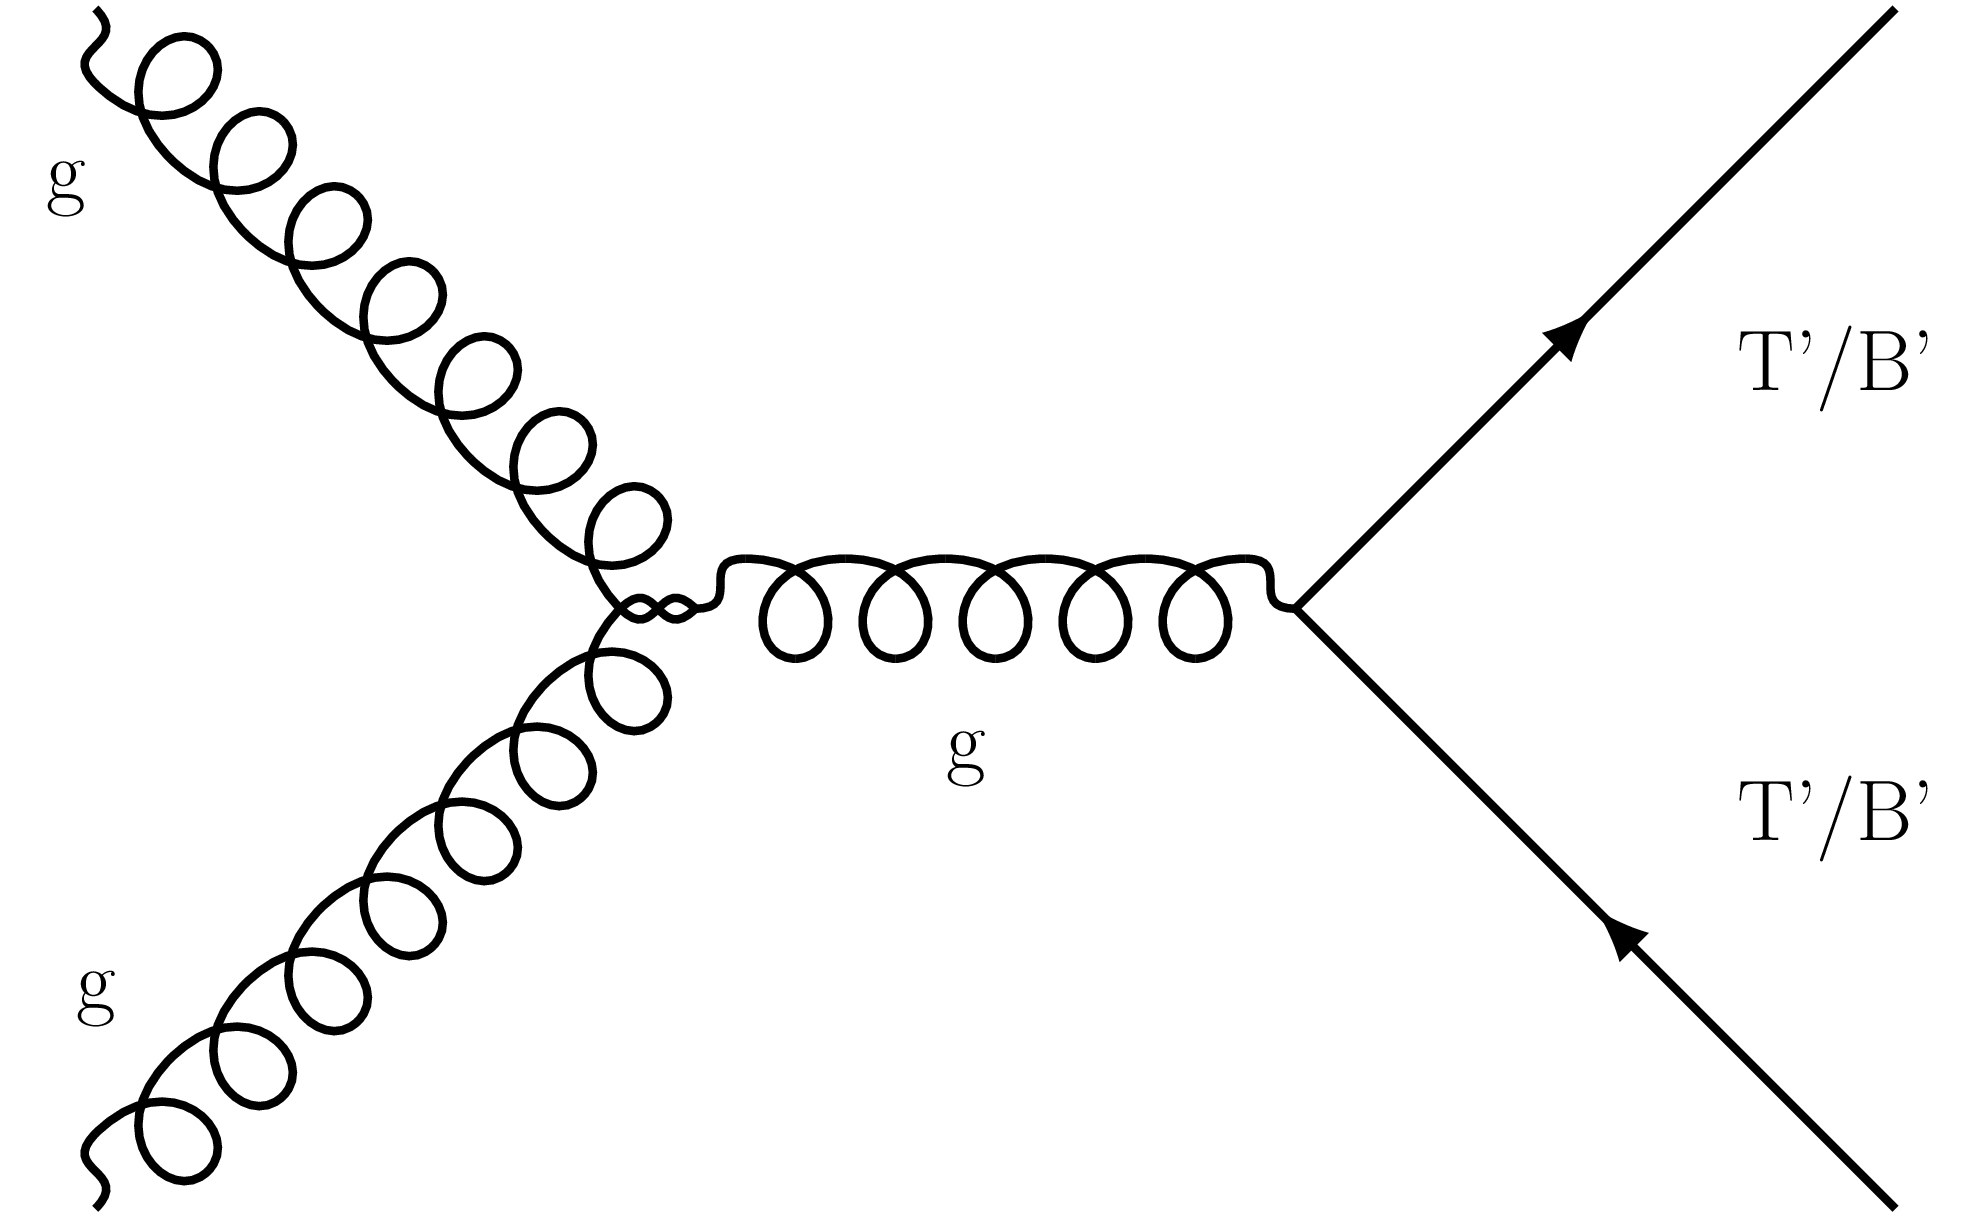
\includegraphics[width=8cm]{Pair Production of VLQs (1).png}
    \caption{Pair production of VLQs. }
    \label{fig:VLQpairprod}
\end{figure}
